\documentclass[conference]{IEEEtran}
\IEEEoverridecommandlockouts
% The preceding line is only needed to identify funding in the first footnote. If that is unneeded, please comment it out.
\usepackage{cite}
\usepackage{amsmath,amssymb,amsfonts}
\usepackage{algorithmic}
\usepackage{graphicx}
\usepackage{textcomp}
\usepackage{xcolor}
\def\BibTeX{{\rm B\kern-.05em{\sc i\kern-.025em b}\kern-.08em
    T\kern-.1667em\lower.7ex\hbox{E}\kern-.125emX}}
\begin{document}

\title{Sentiment Analysis Using LSTM\\
\thanks{Identify applicable funding agency here. If none, delete this.}
}

\author{\IEEEauthorblockN{1\textsuperscript{st}Kunal Rai}
\IEEEauthorblockA{\textit{ Department of Computer Science and Engineering} \\
\textit{ National Institute of Technology Uttarakhand,}\\
 kunalrai.cse16@nituk.ac.in \\}
}

\maketitle

\begin{abstract}
The rise of social media in couple of years has changed the general perspective of networking, socialization, and
personalization. Use of data from social networks for different purposes, such as election prediction, sentimental analysis, marketing, communication, business, and education, is increasing day by day. Precise extraction of valuable information from short text messages posted on social media (IMDB) is a collaborative task. In this paper, we analyze movie reviews to classify data and sentiments from IMDB more precisely. The information from movie reviews are extracted using keyword based knowledge extraction. Moreover, the extracted knowledge is further enhanced using domain specific seed based enrichment technique. The proposed methodology facilitates the extraction of keywords, entities, synonyms, and parts of speech from reviews using LSTM architecture which are then used for reviews classification and sentimental analysis. Dataset of 50,000 movies reviews from IMDB, labeled by sentiment (positive/negative). Reviews have been preprocessed, and each review is encoded as a sequence of word indexes (integers).
\end{abstract}

\begin{IEEEkeywords}
Sentimental Analysis,LSTM,IMDB
\end{IEEEkeywords}

\section{Introduction}

What different human beings assume has continually been an crucial piece of statistics for most of us for the duration of the choice-making manner. Long before attention of the World Wide Web became large, lots of us asked our pals to propose a car mechanic or to give an explanation for who they have been planning to vote for in neighborhood elections, asked reference letters regarding process candidates from colleagues, or consulted Consumer Reports to decide what dishwasher to buy. But the Internet and the Web have now (among other things) made it viable to discover approximately the reviews and studies of those inside the massive pool of human beings that are neither our personal associates nor famous professional critics —that is, people we've got by no means heard of. And conversely, increasingly people are making their evaluations to be had to strangers via the Internet.

According to 2 surveys of more than 2000 American adults each [5,6], 

• 81\% of Internet users (or 60\% of Americans) have finished on-line research on a product at least once;

 • 20\% (15\% of all Americans) do so on a normal day; 

• Amongst readers of on line critiques of restaurants, accommodations, and numerous offerings (e.G., tour businesses or doctors), between 73\% and 87\% report that reviews had a sizable influence on their purchase; 

• Consumers document being inclined to pay from 20\% to  99\% greater for a 5-superstar-rated object than a 4-celebrity-rated object (the variance stems from what form of item or provider is considered); 

• 32\% have provided a rating on a product, carrier, or individual through an internet ratings gadget, and 30\% (inclusive of 18\% of on-line senior citizens) have published an online remark or evaluation regarding a services or products. 

The person hunger for and reliance upon on line advice and tips that the information above famous is simply one motive at the back of the surge of hobby in new systems that deal immediately with reviews as a first-class object. But, Horrigan [6] reports that even as a majority of American net customers record high-quality studies all through on line product studies, on the same time, fifty eight% also report that on-line records was lacking, impossible to discover, confusing, and/or overwhelming. Thus, there's a clear need to useful resource purchasers of merchandise and of information through building better statistics-get right of entry to systems than are presently in lifestyles. 

Marketers have always had to display media for facts associated with their brands — whether or not it’s for public relations activities, fraud violations,3 or competitive intelligence. But fragmenting media and converting customer behavior have crippled traditional tracking strategies. Technorati estimates that 75,000 new blogs are created daily, along with 1.2 million new posts every day, many discussing customer opinions on products and services. Tactics [of the traditional sort] together with clipping services, field marketers, and advert hoc research genuinely can’t hold pace

 - Kim[4]

 Thus, apart from people, an extra audience for structures able to mechanically studying client sentiment, as expressed in no small element in on-line venues, are organizations traumatic to apprehend how their services and products are perceived.

 In this paper we observe a famous movie overview website IMDB to acquire reviews and classify them into  training this is "advantageous" or "negative" primarily based on the opinion provided by means of the person. This generation can assist users who need to recognise what's the overall response of the humans who have seen the film. We have constructed a LSTM(Long Short Term Memory) version of Recurrent Neural Network to classify the film evaluations into  training i.E. Fine or poor.An IMDB movie overview dataset with 50,000 film evaluations has been used to teach and take a look at this model.

\section{Background}

\subsection{Neural Network Text Classification}\label{AA}

 When given textual data, a general objective is to classify
the data for analytical or statistical purposes. Text
classification is performed in [33], while [34] and [35]
performed sentiment categorization, all on social media datasets
using neural networks. In [31] and [36] authors compared
multiple techniques on the sentiment analysis
of movie review. In [31] authors compared multiple n-gram
machine learning approaches on the IMDb sentiment
dataset used in this paper. The data was preprocessed before
being vectorized and trained into various configuration of machine
learning algorithms. Many of these techniques in [31] reached
good accuracies in the 80\% with the best configuration
“Unigram + Bigram + Trigram” reaching the maximum
accuracy of 88.94\%. 

\subsection{Word Level Text Classification}\label{AA}

Word-Level Text Classification is a more traditional
technique to textual content classfication with neural networks. Authors in
[37] created a shallow CNN that classifies using more than one
distinctive kernels. In this community, a convolutional layer will
study n words at a time while applying the filters and
pooling-over-time. The community would use a couple of kernel
sizes and concatenate the effects; consequently, the network finds
context from the n range of words nearby the word. The
very last connected layer makes use of this information for category.
This community is simple but effective in textual class.
Authors in [30] use IMDb evaluate facts with a new LSTM
neural community to categorise sentiment of the assessment. The evaluate
facts contained no impartial information. The dictionary became restrained to
the pinnacle 2000 most used phrases and every evaluation collection turned into
capped at a hundred phrases and padded with zeros if less than the
max. The proposed LSTM layer is a biologically-stimulated
additive version of a traditional LSTM that produced higher
loss balance, however lower accuracy. The quality accuracy carried out
between both LSTM models turned into nonetheless below 85%. The use of
an LSTM on textual records offers better contextual view of
phrases than a CNN.


\subsection{Dataset}
To achieve best results , we need a reliable dataset with genuine reviews from actual movie watchers and hence, we can't use reviews from any unknown source. News channels also provide movie reviews on new movies every week but we can't trust the biased nature of these movie reviews since the movie makers can influence these channels in lieu of advertisement in their movie or sponsorship for their channel or any connection with the actors in the movie.

\begin{figure}[htbp]
\centerline{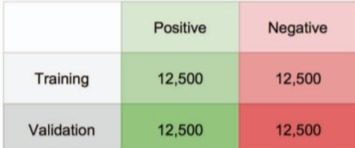
\includegraphics[width=80mm,scale=0.6]{6.jpg}}
\caption{Distribution of dataset.}
\label{fig}
\end{figure}

Therefore, due to above apprehensions , we have used the IMDB(Internet Movie Database)[21] website for unbiased movie reviews which are written by normal movie go-ers like us who don't have any bias in their movie reviews . This will help us provide an accurate and unbiased general opinion of the audience about the movie and will help the makers to make necessary changes in their next venture.

The ACL Internet Movie Database (IMDb) dataset used changed into created in [3] for gaining knowledge about phrase vectors. The dataset consists of 50,000 textual evaluations of movies; half (25,000) of the reviews are for trying out and have no label. The other (25,000) opinions are paired with a label of zero or 1 to represent negative and nice sentiment, respectively. These labels had been linearly mapped from the IMDb’s rating system in which reviewers can rate a movie a fixed range of stars from 1 to 10. Fig. 1 illustrates the business enterprise of the dataset. The evaluations with labels are cut up in half; every set has 12,500 effective evaluations and 12,500 bad opinions to maintain the facts balanced.

\begin{figure}[htbp]
\centerline{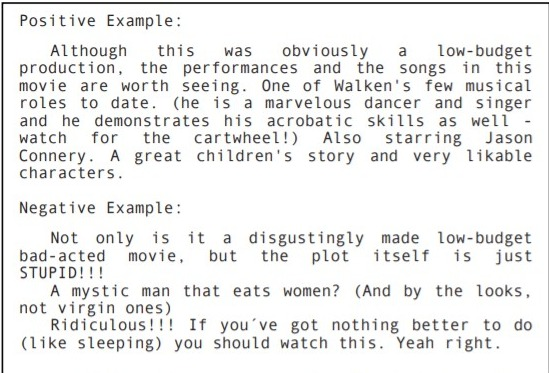
\includegraphics[width=80mm,scale=0.6]{7.jpg}}
\caption{An example from the dataset.}
\label{fig}
\end{figure}

\end{itemize}

\section{Related Work}
Although the region of sentiment analysis and opinion mining has lately loved a large burst of research pastime, there was a steady undercurrent of hobby for pretty a while. One ought to count number early tasks on ideals as forerunners of the location [3, 2]. Later work focused totally on interpretation of metaphor, narrative, point of view, affect, evidentiality in text, and associated areas [1,7,8,9,10,11,12,13,14].

The 12 months 2001 or so seems to mark the start of tremendous attention of the studies issues and opportunities that sentiment evaluation and opinion mining increase [15, 16, 17, 18,19], and eventually there were actually hundreds of papers posted on the situation.

Factors at the back of this “land rush” consist of:

• The upward thrust of gadget mastering methods in herbal language
processing and facts retrieval;

• The availability of datasets for device mastering algorithms
to be trained on, because of the blossoming of the World Wide
Web and, in particular, the improvement of evaluate-aggregation
web-sites; and, of course

• Realization of the charming intellectual demanding situations and industrial and intelligence programs that the location offers.

The term opinion mining appears in a paper by Dave et al. That became posted inside the proceedings of the 2003 WWW conference; the booklet venue may also give an explanation for the popularity of the term inside communities strongly related to Web search or records retrieval. According to Dave et al., the precise opinion-mining tool might “technique a hard and fast of search results for a given item, producing a listing of product attributes (first-rate, features, and many others.) and aggregating evaluations approximately every of them (terrible, mixed, exact).” Much of the subsequent research self-diagnosed as opinion mining fits this description in its emphasis on extracting and reading judgments on numerous factors
of given items. However, the term has currently additionally been interpreted more extensively to consist of many one of a kind varieties of analysis of evaluative text .
The records of the word sentiment evaluation parallels that of “opinion mining” in certain respects. The term “sentiment” used in reference to the automatic analysis of evaluative text and tracking of the predictive judgments therein appears in 2001 papers by means of Das and Chen and Tong , due to these authors’ interest in reading marketplace sentiment. It finally happened within 2002 papers by means of Turney and Pang et al., which were posted inside the proceedings of the once a year meeting of the Association for Computational Linguistics (ACL) and the yearly conference on Empirical Methods in Natural Language Processing (EMNLP). Moreover, Nasukawa and Yi [20] entitled their 2003 paper, “Sentiment evaluation: Capturing favorability the use of natural language processing”, and a paper in the equal yr by Yi et al.  Became named “Sentiment Analyzer: Extracting sentiments approximately a given topic using herbal language processing techniques.” These activities collectively may additionally provide an explanation for the popularity of “sentiment analysis” among groups self-recognized as centered on NLP. A substantial variety of papers mentioning “sentiment evaluation” consciousness on the precise software of
classifying opinions as to their polarity (both advantageous or terrible), a reality that appears to have brought about a few authors to signify that the word refers specially to this narrowly described mission. However, nowadays many construe the time period extra widely to intend the computational remedy of opinion, sentiment, and subjectivity in text.


\section{Proposed Method}
There are several objectives driving the current study. One goal is to provide a guideline for movie makers
that want to have a better understanding of how their movie is received by their customers and also what is
the attitude towards their product. Such information is necessary for successful decision making,
as it can give the maker an objective understanding of the customers’ opinions. This knowledge can be applied in improving the success rate of movie maker and the movies. It can also be used to customize specific parts or genres and target them to a more appropriate movie watchers.

The sentiment analyzers in the past have been built using the K-means,t-Stochastic Neighbourhood Embedding,Tf-Idf word2vector or Naive Bayes techniques that have produced acceptable results but we have here used the Recurrent Neural Network model to retain memory of the sentences in the review.

\subsection{Preprocessing for input in the model}
Before providing the corpus of words and giving input in our RNN model , we have provided padding in the embedding matrix so that we don't miss out on any important words at the beginning or end of the sentences.

\subsection{Architecture of the RNN model}
 We are aware that using simple Recurrent Neural Network architecture can result in either vanishing gradient or exploding gradient problem and hence the results are not very accurate or convincing. To deal with this problem we have used the LSTM(Long Short Term Memory) architecture to solve the vanishing gradient problem. 

Along with the output from previous layer and input from the current layer which is used in the normal Recurrent Neural Network model , we also use the memory unit from previous layer which accumulates the result of all previous layers as input to the current layer.

Our model classifies the reviews in two classes - "positive" and "negative" . We believe that neutral reviews don't really affect the overall general opinion of the audience and they are not useful to the movie makers either as they are looking for criticism so that they can improve the next time they start making a movie.

We have used an LSTM of one hundred units because most of the movie goers who write a review don't write a movie review of more than 100 words and hence, having a memory unit of around one hundred words is sufficient to achieve the correct result and classify the movie review into a 'positive' or a 'negative' review.

\section{Experiment and Discussion}

Our LSTM(Long Short Term Memory) model was built with the help of keras[22] librabry and Tensorflow framework at the backend[29] to train and use the pre-existing LSTM architecture.We used Google colaboratory environment to train our model wth GPU runtime environment.

We took a vocabulaory size of 5000 words to train the model. We use this vocabulory to build Word Embeddings[23] and Embedding Matrix[24] .

Preprocessing of the dataset is done to provide padding so that we don't miss out on important data which can change the sentiment of the review .

\begin{figure}[htbp!]
\centerline{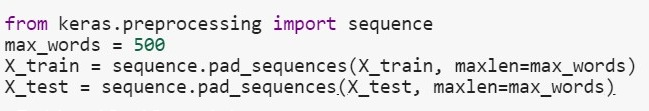
\includegraphics[width=80mm,scale=0.6]{1.jpg}}
\caption{Preprocessing of the dataset(Padding).}
\label{fig}
\end{figure}

\subsection{Accuracy and Comparison}

The achieved accuracy surpassed other models’ results on
the same IMDb review sentiment dataset. Both the traditional
and the proposed LSTM models in [30] plateaued at an accuracy
just over 80\%, with a maximum under 85\%. The accuracy in
[30] was used as a baseline accuracy for a simple, lone LSTM
model. Our model’s performance can also be compared to
other machine learning methods. Authors in [32] proposed a
hybrid supervised-unsupervised model when they created the
IMDb review sentiment dataset. Their highest reported
accuracy was 88.89% from their full model with additional
unlabeled reviews and bag of words vectors. Authors in [31]
experimented with multiple variation of machine learning
models on the IMDb dataset. The best accuracy achieved in [31]
was 85.94\% from their combined Unigram-Bigram-Trigram
model. From reviewing these other machine learning models, it
is clear that our proposed method outperforms prior work

\subsection{Architecture of the LSTM model}

We have built a sequential neural net[25] which considers the output of last layer and input of current layer to produce output.

In a single uint of our recurrent neural network their is a LSTM architecture unit and at the end of the model is the softmax[26] layer which uses the sigmoid activation function[8] for output. There are one hundred such LSTM units for one hundred words in one iteration and if the review is longer than one hundred words , we take the final state of memory of previous iteration as the initial input of the next iteration so that iteration can co-relation between words can be deduced and hence the correct sentiment can be achieved. 

Our model outputs 0 for 'negative' and 1 for 'positive' sentiment of the movie review. Architecture of our model is shown in the image below-

\begin{figure}[htbp!]
\centerline{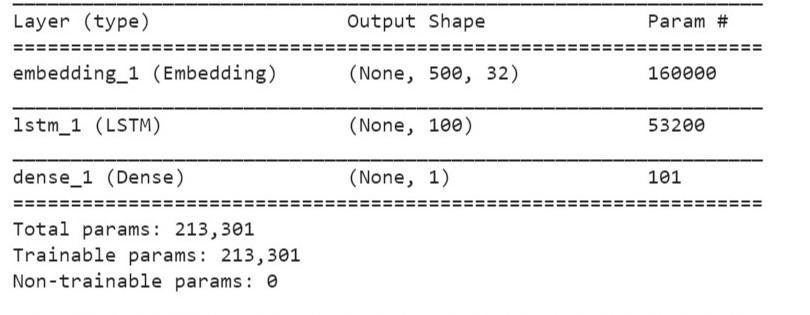
\includegraphics[width=80mm,scale=0.5]{4.jpg}}
\caption{Architecture of the RNN.}
\label{fig}
\end{figure}

We trained our model on 25,000 out of the 50,000 movie reviews with 10 epochs and batch size (i.e. number of words in one iteration of the epoch) of 48 words. Below I have shown the 10 epochs of the training which show increasing accuracy  , we have also shown the loss and accuracy after each epoch and it is evident that the results are approching the maxima as the accuracy is  strictly increasing.

\begin{figure}[htbp!]
\centerline{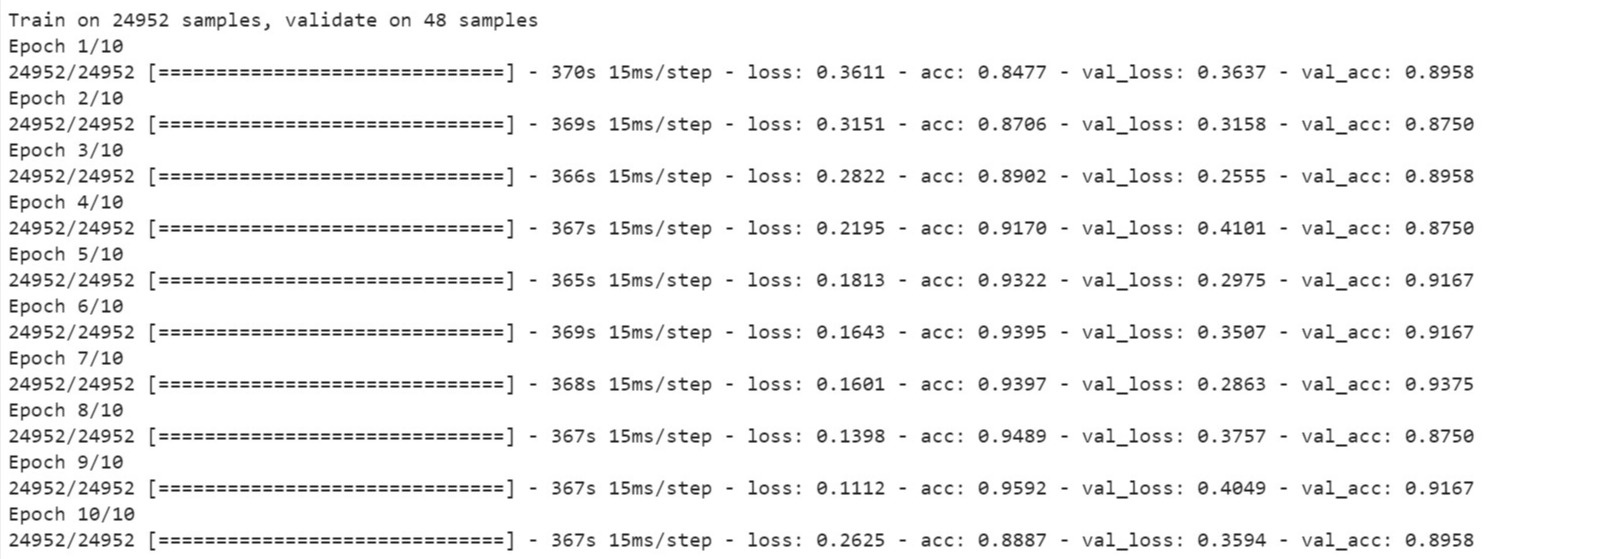
\includegraphics[width=90mm,scale=1]{10.jpg}}
\caption{First 3 epochs with accuracy measure and loss measure.}
\label{fig}
\end{figure}

Below is the graph plot for the accuracy-

\begin{figure}[htbp!]
\centerline{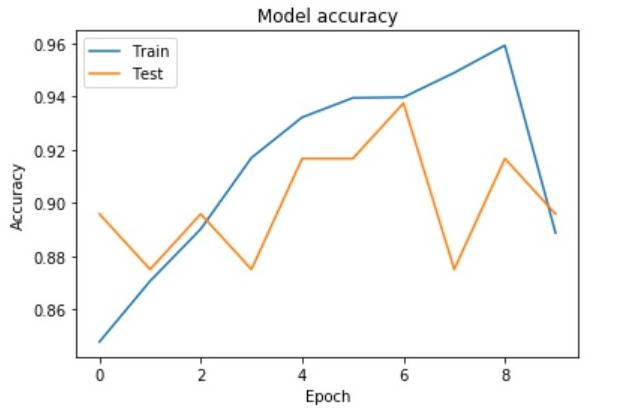
\includegraphics[width=90mm,scale=1]{8.jpg}}
\caption{Model Accuracy.}
\label{fig}
\end{figure}

The network is compiled with a binary cross entropy loss
function; this loss calculates loss with two classes (0 and 1).
For this paper’s purposes, 0 represents negative sentiment and
1 represents positive sentiment. The loss is calculated on the
single and final output of the dense layer.
The network is also compiled with an optimizer; Adam was the
optimizers used for testing during the experiments. Each
optimizer was used with varying learning rates and learning
rate decay parameters. 


We have used the 'adam'[27] optimizer to achieve the maxima. The code snippet of the compilation of the model after training is shown below

\begin{figure}[htbp!]
\centerline{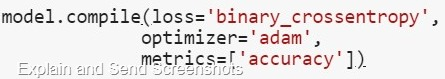
\includegraphics[width=80mm,scale=0.5]{3.jpg}}
\caption{adam used for error optimization.}
\label{fig}
\end{figure}

Below is the graph plot for loss function-

\begin{figure}[htbp!]
\centerline{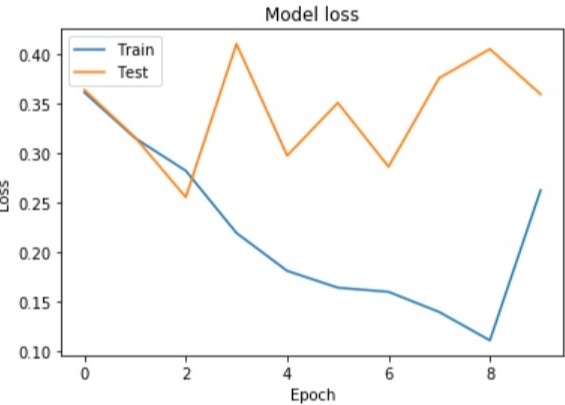
\includegraphics[width=90mm,scale=1]{9.jpg}}
\caption{Model Loss.}
\label{fig}
\end{figure}

Finally , the test result show the accuracy of over 86\% of the model after ten epochs. 

\begin{figure}[htbp!]
\centerline{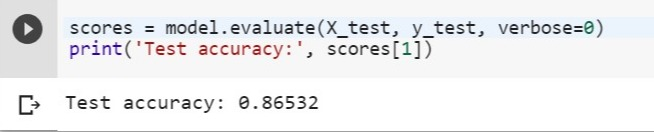
\includegraphics[width=90mm,scale=1]{11.jpg}}
\caption{Final Accuracy.}
\label{fig}
\end{figure}

\section{Conclusions}
We presented results for sentiment analysis on IMDB movie reviews. We first presented the previous/standard work done using K-NN[28] or Naive Bayes techniques and showed that our LSTM model produces higher accuracy with much lesser computation power and iterations. Whn classified using Bag of words using K-NN technique for K=3 , the accuracy was around 78\%. for iterations much greater than 10. In our LSTM model , we got an accuracy of over 86\% with just ten epochs on a dataset with over 25,000 movie reviews. Given more computation power and bigger dataset , we can easily achieve better and more accurate model. 

\section{Future Work}
One region of investigating that would be useful is the use of different varieties of word representations. While the
embedding become used, different techniques, which includes bag of words and TF-IDF, will be jumbled in to provide one of a kind outcomes. While it became established that GoogleNews embeddings from Wiki FastText embeddings did now not add to the accuracy, other pre-trained models can also have better effect. There may also be different pre-processing techniques that might increase the efficacy of the model.

\begin{thebibliography}{00}

\bibitem{foo99:baz99}
M. Hearst,
{\em  “Direction-based text interpretation as an information access
refinement,” in Text-Based Intelligent Systems, (P. Jacobs, ed.), pp. 257–274,
Lawrence Erlbaum Associates, 1992}

\bibitem{foo98:baz98}
Y. Wilks and J. Bien,
{\em “Beliefs, points of view and multiple environments,”
in Proceedings of the international NATO symposium on artificial and human
intelligence, pp. 147–171, USA, New York, NY: Elsevier North-Holland, Inc.,
1984.}

\bibitem{foo97:baz97}
J. Carbonell
{\em  Subjective Understanding: Computer Models of Belief Systems.},
PhD thesis, Yale, 1979.Surveys (CSUR) 11, 4, (1979), pp. 305-330.

\bibitem{foo96:baz96}
 P. Kim,
{\em  “The forrester wave: Brand monitoring", Q3 2006,Forrester Wave (white paper), 2006.},


\bibitem{foo93:baz93}
 J. A. Horrigan
{\em  Online shopping,Pew Internet and American Life Project Report, 2008.}


\bibitem{foo95:baz95}
comScore/the Kelsey group
{\em “Online consumer-generated reviews have significant impact on offline purchase behavior,” Press Release, http://www.
comscore.com/press/release.asp?press=1928, November 2007.},

\bibitem{foo94:baz94}
 A. Huettner and P. Subasic,
{\em  “Fuzzy typing for document management,” in
ACL 2000 Companion Volume: Tutorial Abstracts and Demonstration Notes,
pp. 26–27, 2000.}

\bibitem{foo92:baz92}
M. Kantrowitz,
{\em    “Method and apparatus for analyzing affect and emotion in
text,” U.S. Patent 6622140, Patent filed in November 2000, 2003.}

\bibitem{foo92:baz92}
 W. Sack,
{\em  “On the computation of point of view,” in Proceedings of AAAI,
p. 1488, 1994. (Student abstract).}

\bibitem{foo92:baz92}
 J. Wiebe and R. Bruce,
{\em  “Probabilistic classifiers for tracking point of view,”
in Proceedings of the AAAI Spring Symposium on Empirical Methods in Discourse Interpretation and Generation, pp. 181–187, 1995.}

\bibitem{foo92:baz92}
J.M. Wiebe, 
{\em “Identifying subjective characters in narrative,” in Proceedings
of the International Conference on Computational Linguistics (COLING),
pp. 401–408, 1990.}

\bibitem{foo92:baz92}
 J. M. Wiebe,
{\em ]  “Tracking point of view in narrative,” Computational Linguistics,
vol. 20, pp. 233–287, 1994.}

\bibitem{foo92:baz92}
J. M. Wiebe, R. F. Bruce, and T. P. O’Hara,
{\em ]   “Development and use of a
gold standard data set for subjectivity classifications,” in Proceedings of the
Association for Computational Linguistics (ACL), pp. 246–253, 1999.}

\bibitem{foo92:baz92}
J. M. Wiebe and W. J. Rapaport,
{\em ]   “A computational theory of perspective and
reference in narrative,” in Proceedings of the Association for Computational
Linguistics (ACL), pp. 131–138, 1988.}

\bibitem{foo92:baz92}
 C. Cardie, J. Wiebe, T. Wilson, and D. Litman,
{\em ]  “Combining low-level and
summary representations of opinions for multi-perspective question answering,” in Proceedings of the AAAI Spring Symposium on New Directions in
Question Answering, pp. 20–27, 2003}

\bibitem{foo92:baz92}
  S. Das and M. Chen,
{\em ] “Yahoo! for Amazon: Extracting market sentiment from
stock message boards,” in Proceedings of the Asia Pacific Finance Association
Annual Conference (APFA), 2001.}

\bibitem{foo92:baz92}
   K. Dave, S. Lawrence, and D. M. Pennock,
{\em ]  “Mining the peanut gallery: Opinion extraction and semantic classification of product reviews,” in Proceedings
of WWW, pp. 519–528, 2003.}

\bibitem{foo92:baz92}
   L. Dini and G. Mazzini, 
{\em ]“Opinion classification through information extraction,” in Proceedings of the Conference on Data Mining Methods and
Databases for Engineering, Finance and Other Fields (Data Mining),
pp. 299–310, 2002}

\bibitem{foo92:baz92}
    H. Liu, H. Lieberman, and T. Selker,
{\em ]  “A model of textual affect sensing using
real-world knowledge,” in Proceedings of Intelligent User Interfaces (IUI),
pp. 125–132, 2003.}

\bibitem{foo92:baz92}
     T. Nasukawa and J. Yi, 
{\em ] “Sentiment analysis: Capturing favorability using
natural language processing,” in Proceedings of the Conference on Knowledge
Capture (K-CAP), 2003.}

\bibitem{foo92:baz92}
IMDB-
{\em https://www.imdb.com/}


\bibitem{foo92:baz92}
Keras-
{\em https://keras.io/}


\bibitem{foo92:baz92}
Word Embeddings-{\em https://machinelearningmastery.com/what-are-word-embeddings/}

\bibitem{foo92:baz92}
Embedding Matrix-
{\em https://www.coursera.org/lecture/nlp-sequence-models/embedding-matrix-K604Z}

\bibitem{foo92:baz92}
Sequence Models-
{\em https://medium.com/machine-learning-bites/deeplearning-series-sequence-models-7855babeb586}

\bibitem{foo92:baz92}
Softmax-
{\em https://developers.google.com/machine-learning/crash-course/multi-class-neural-networks/softmax}

\bibitem{foo92:baz92}
adam algorithm-
{\em https://machinelearningmastery.com/adam-optimization-algorithm-for-deep-learning/}

\bibitem{foo92:baz92}
K-Neighbours Algorithm-
{\em https://www.analyticsvidhya.com/blog/2018/03/introduction-k-neighbours-algorithm-clustering/}

\bibitem{foo92:baz92}
Tensorflow-
{\em https://www.tensorflow.org/}

\bibitem{foo92:baz92}
L. Rahman, N. Mohammed, and A. Kalam Al Azad,
{\em  "A new LSTM
model by introducing biological cell state." In Electrical Engineering
and Information Communication Technology (ICEEICT), 2016 3rd
International Conference on, pp. 1-6, 2016}

\bibitem{foo92:baz92}
A. Tripathy, A. Agrawal, and S. Kumar Rath,
{\em  "Classification of
sentiment reviews using n-gram machine learning approach." Expert
Systems with Applications, vol. 57, pp. 117-126, 2016. }

\bibitem{foo92:baz92}
 A.L. Maas, R.E. Daly, P.T. Pham, D. Huang, A.Y. Ng, and C. Potts,
{\em
"Learning word vectors for sentiment analysis." In Proceedings of the
49th Annual Meeting of the Association for Computational Linguistics:
Human Language Technologies, vol.1, pp. 142-150, 2011.}

\bibitem{foo92:baz92}
 F. Sebastiani,
{\em
 "Machine learning in automated text categorization," ACM
computing surveys (CSUR), vol. 34, no. 1, pp 1-47, 2002. }

\bibitem{foo92:baz92}
 L. Chen, C. Liu, and H. Chiu,
{\em
 "A neural network based approach for
sentiment classification in the blogosphere," Journal of Informetrics,
vol. 5, no. 2, pp. 313-322, 2011. }

\bibitem{foo92:baz92}
 A. Severyn, and A. Moschitti, 
{\em
 "Unitn: Training deep convolutional
neural network for twitter sentiment classification," In Proceedings of
the 9th International Workshop on Semantic Evaluation (SemEval
2015), Association for Computational Linguistics, Denver, Colorado, pp.
464-469. 2015. }

\bibitem{foo92:baz92}
B. Pang, L. Lee, and S. Vaithyanathan,
{\em
 "Thumbs up?: sentiment
classification using machine learning techniques," In Proceedings of the
ACL-02 conference on Empirical methods in natural language
processing, vol. 10, pp. 79-86, 2002.}

\bibitem{foo92:baz92}
 Y. Kim,
{\em
 "Convolutional neural networks for sentence classification,"
arXiv preprint arXiv:1408.5882, 2014. }

\end{thebibliography}
\vspace{12pt}
\end{document}
